\documentclass[twocolumn,preprintnumbers,amsmath,amssymb,notitlepage,nofootinbib,longbibliography,superscriptaddress,aps,pra,10pt]{revtex4-1}
% \documentclass[a4paper,twocolumn,superscriptaddress,amsmath,amssymb,longbibliography,10pt]{quantumarticle}

% Packages and custom commands
	\usepackage{natbib}
	\usepackage{graphicx}
	\usepackage{dcolumn}
	\usepackage{dsfont}
	\usepackage{bm}

	\usepackage{times}

	\usepackage{amsmath}

	%\usepackage{float}


	\usepackage[usenames, dvipsnames]{color}
	\usepackage{url}
	\usepackage[colorlinks=true,breaklinks=true,allcolors=blue]{hyperref}
	% \usepackage{hyperref}
	\usepackage{microtype}

	\newtheorem{theorem}{Theorem}
	\newtheorem{lemma}{Lemma}

	\newcommand{\ryan}[1]{\textcolor{cyan}{RS: #1}}

	\newcommand{\mk}[1]{\textcolor{cyan}{MK: #1}}

	\newcommand{\en}[1]{\textcolor{cyan}{EN: #1}}

	\newcommand{\je}[1]{\textcolor{cyan}{#1}}

\begin{document}

% Title page
	\title{DeepQ \je{machine learning} decoding for fault tolerant quantum computation}

	\author{Ryan Sweke}
	\affiliation{\mbox{Dahlem Center for Complex Quantum Systems, Freie Universit\"{a}t Berlin, 14195 Berlin, Germany}}
	\author{Markus S. Kesselring}
	\affiliation{\mbox{Dahlem Center for Complex Quantum Systems, Freie Universit\"{a}t Berlin, 14195 Berlin, Germany}}
	\author{Evert P.~L. van Nieuwenburg}
	\affiliation{\mbox{Institute for Quantum Information and Matter, Caltech, Pasadena, CA 91125, USA}}
	\author{Jens Eisert}
	\affiliation{\mbox{Dahlem Center for Complex Quantum Systems, Freie Universit\"{a}t Berlin, 14195 Berlin, Germany}}


	\date{\today}

% Abstract
	\begin{abstract}
		Topological error correcting codes, and particularly the surface code, currently provide the most feasible 
		roadmap towards large-scale fault tolerant quantum computation.
		As such, obtaining fast and flexible decoding algorithms for these codes, within the experimentally relevant context 
		of faulty syndrome measurements, is of critical importance.
		In this work, we show that the problem of decoding such codes, in the full fault tolerant setting, can be naturally reformulated as a process of 
		repeated interactions between a decoding agent and a code environment, to which the machinery of reinforcement learning 
		can be applied to obtain decoding agents.
		As a demonstration, by using deepQ learning, we obtain fast decoding agents for the surface code, for a variety of 
		\je{natural} noise-models.
		%, within the fully fault tolerant setting.
		 \je{We argue that it is specifically the practically important situation of fault tolerant decoding that is particularly suitable
		 to be tackled with notions of reinforcement learning.}
		%We argue that this problem is specifically suitable to be tackled with notions of reinforcement learning.
	\end{abstract}

\maketitle

\section{Introduction}\label{s:introduction}
	In order to implement large scale quantum \je{computations} it is necessary to be able to store and manipulate quantum information in a manner that is robust to the unavoidable errors introduced through interaction of the physical qubits with a noisy environment.
%	A possible strategy
	\je{The known strategy} for achieving such robustness is to encode a single logical qubit into the state of many physical qubits, via a quantum error correcting code, from which it 
	%may be 
	\je{is} possible to actively diagnose and correct errors that may occur~\cite{Terhal15,Campbell17}.
	While many quantum error correcting codes exist, topological quantum codes~\cite{Kitaev03, Dennis02, Preskill17lectures, Nayak08, Pachos12, Terhal15, Brown16, Campbell17}, in which only local operations are required to diagnose and correct errors, are of particular interest as a result of their experimental feasibility~\cite{Reed12, Barends14, Nigg14, Corcoles15, Albrecht16, Takita16, Linke17}.
	%Recently 
	\je{In particular,} the surface code has emerged as an especially promising candidate for large-scale fault-tolerant quantum computation, due to the combination of its comparatively low overhead and locality requirements, coupled with the availability of convenient strategies for the implementation of all required logical gates \cite{Fowler18,Litinski18b}. \je{In fact, road maps towards realizing robust quantum computing focus on achieving this goal based on such surface codes as the 
	most feasible way forward known}.

	\je{The known realistic topological quantum error correcting codes are not self-correcting, however, a feature which comes at a price: They are not robust
	to natural thermal noise. For this reason one has to actively correct for errors following sophisticated prescriptions. That is to say,} in any code-based strategy for fault tolerant quantum computation, decoding algorithms play a critical role.
	At a high level, these algorithms take as input the outcomes of syndrome measurements (which provide a diagnosis of errors that \je{have} occurred on the physical qubits), and provide as output a suggestion of corrections for any errors that may have occurred during the computation. \je{They have to be extremely 
	fast -- faster than the quantum noise can act -- and reliable,
	and as such constitute a serious bottleneck in the realization of fault tolerant quantum computers.}

	It is particularly important to note that in any physically realistic setting, the required syndrome measurements are obtained via small quantum circuits, and are therefore also generically faulty 
	As such, while the setting of perfect syndrome measurements provides a good test-bed for the development of decoding algorithms, any decoding algorithm which aims to be experimentally useful should also be capable of dealing with such faulty syndrome measurements.
	Additionally, such algorithms should also be capable of dealing with experimentally relevant noise models, as well as be fast enough to not present a bottleneck to the execution of computations, even as the size of the system (i.e. the code distance) grows.

	Due to the importance of decoding algorithms for fault tolerant quantum computation, many different approaches have been developed, each of which tries to satisfy as many of the experimentally required criteria as possible.
	Perhaps most prominent are algorithms based on minimum-weight perfect matching subroutines~\cite{Fowler13}, although alternative approaches based on techniques such as the renormalization group~\cite{Duclos2010} and locally operating cellular automata~\cite{Herold15,herold2017cellular,Kubica2018} have also been put forward.

	Recently, techniques from machine learning have begun to find application in diverse areas of quantum physics - such as in the efficient representation of many-body quantum states \cite{WFcarleo2017solving,WFcarleo2018constructing,WFgao2017efficient}, the identification of phase transitions \cite{PTvan2017learning,PTPhysRevB.97.134109,PTcarrasquilla2017machine}, and the autonomous design of novel experimental set-ups \cite{melnikov2018active} - and various neural-network based decoders have also been proposed~\cite{Torlai10, Varsamopoulos17, Krastanov17, Breuckmann18, Baireuther18a, Baireuther18b, Ni18, chamberland2018deep}.
	Despite this diversity of proposed decoding algorithms, there is as of yet no algorithm which clearly satisfies all the required experimental criteria listed above.
	While previously proposed neural network decoders promise extremely fast decoding times \cite{chamberland2018deep}, flexibility with respect to the underlying code and noise model \cite{chamberland2018deep, Breuckmann18} and the potential to scale to large code distances \cite{Ni18}, most neural network decoders are so far restricted to the setting of perfect syndrome measurements.
	Neural network decoders taking faulty syndrome measurements into account~\cite{Baireuther18a,Baireuther18b} currently restrict themselves to the setting of preserving a logical qubit for as long as possible, without the requirement of performing a subsequent logical gate.
	As such, while neural network based approaches to decoding seem promising, there remains room for improvement and new techniques.

	Simultaneously, the last few years have also seen impressive advances in the development of deep reinforcement learning algorithms, which have allowed for the training of neural network based agents capable of obtaining super-human performance in domains such as Atari~\cite{RLMnih15,RLschaul2015prioritized,RLvan2016deep,RLwang2015dueling}, Chess~\cite{RLsilver2017mastering} and Go~\cite{RLSilver2016,RLSilver17b}.
	These techniques are particularly powerful in situations where it is necessary to learn strategies for complex sequential decision making, involving consideration of the future effects of ones actions.
	In this work we demonstrate that decoding in the context of fault-tolerant quantum computing provides a natural setting for the application of reinforcement learning methods.
	We will discuss the advantages of such an approach over the previously proposed neural network decoders.

	In particular, we interpret the decoder as an agent performing discrete, sequential actions on an environment which is defined by a quantum error correction code.
	This conceptual framework allows for the application of various deep reinforcement learning algorithms to obtain neural network based decoding agents.
	As a demonstration, we then utilize to deepQ learning to obtain fast surface code decoders, for a variety of noise models, in the fully fault-tolerant setting.
	These results provide a foundation for extension via both more sophisticated reinforcement learning techniques and neural network models.

	In this work we begin by providing an introductory overview of the surface code in Section~\ref{s:the_surface_code}, before presenting a description of the decoding problem for fault-tolerant quantum computation in Section~\ref{s:the_decoding_problem}.
	After a brief introduction to the formalism of reinforcement learning and $Q$-functions in Section~\ref{s:reinforcement_learning} we are then able to provide the conceptual reframing of decoding as a reinforcement learning problem in Section~\ref{s:decoding_as_rl}, representing one of the primary results of this work.
	In Section~\ref{s:results} we then present deepQ surface code decoders for a variety of noise models, before finally in Section~\ref{s:conclusions} we discuss both the advantages and disadvantages of the approach presented here, along with various potential strategies for building upon the results presented in this work.

\section{The Surface Code}\label{s:the_surface_code}

	We begin by providing a brief description of the surface code.
	The framework and methods presented in this work are not restricted to the surface code however, and may be applied to any stabilizer code.
	The restriction to the surface code is made both for simplicity of presentation and experimental relevance.
	We will focus on presenting the essential elements of the surface code and refer to more complete treatments for details \cite{Gottesman97, Terhal15,Litinski18b}.

	We will consider $d\times d$ lattices with a \textit{physical} data qubit on each vertex $v$, as illustrated in Fig.~\ref{f:surface_code} for $d=5$.
	The collective state of all qubits on the lattice is an element of the Hilbert space $\mathcal{H} = \mathbb{C}^{2^{(d\times d)}}$.
	We associate stabilizer operators with each coloured plaquette of the lattice.
	Stabilizers on blue (orange) plaquettes are operators which apply Pauli $X$ ($Z$) flips to all qubits on the vertices of the plaquette.
	Specifically, denoting the set of all blue (orange) plaquettes as $B_p$ ($O_p$) we define the stabilizer $S_p$ on plaquette $p$ as,

	\begin{equation}\label{e:stabilizer_definition}
		S_p = \bigotimes_{v\in p} \sigma_v \quad \text{where }
		\begin{cases}
			\sigma_v = X_v \quad \text{if } p \in B_p,\\
			\sigma_v = Z_v \quad \text{if } p \in O_p.
		\end{cases}
	\end{equation}
	All stabilizers are mutually commuting and have eigenvalues $\pm 1$.
	This allows for the introduction of a  Hamiltonian $H = -\sum_p S_p$ from which the surface code $\mathcal{H}_\mathrm{sc} \subset \mathcal{H}$ is defined to be the ground state space of $H$.
	Alternatively, this space consists of all simultaneous $+1$ eigenstates of all stabilizers.
	This subspace is two dimensional, i.e. $\mathcal{H}_\mathrm{sc} \simeq \mathbb{C}^2$, and hence can encode a single \textit{logical} qubit.
	Logical operators are operators which preserve the code space, and can therefore be used to manipulate the state of the logical qubit.
	Fig.~\ref{f:surface_code} shows logical $X$ ($Z$) operators, denoted $X_L$ ($Z_L$), which are continuous strings of single vertex $X$ ($Z$) operators connecting the top and bottom (left and right) boundaries of the lattice.

	\begin{figure}
		\centering
		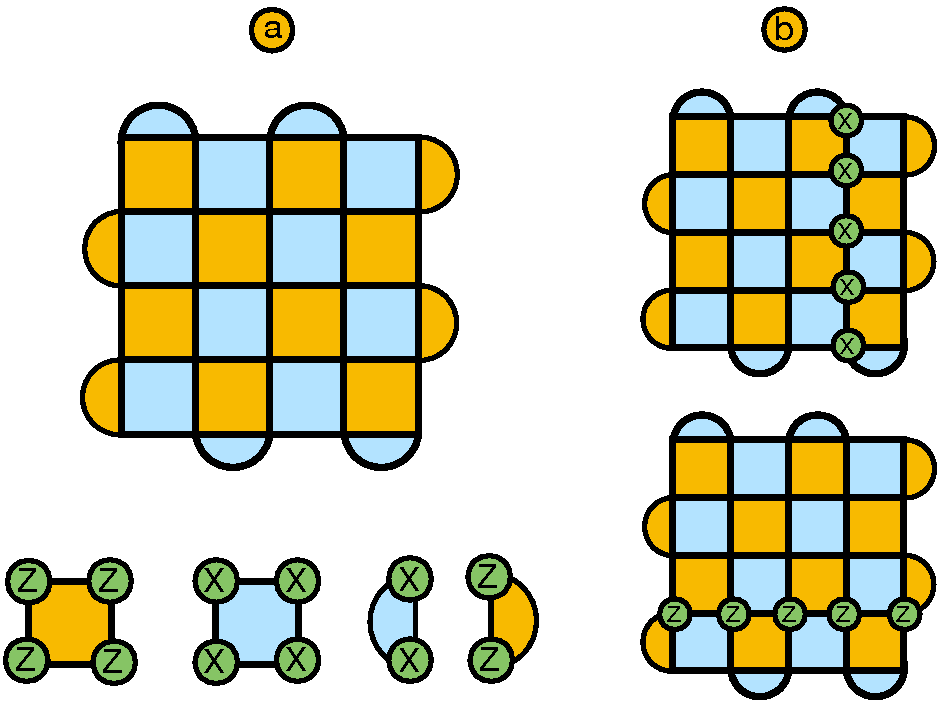
\includegraphics[width=0.8\linewidth]{figures/surface_code.pdf}
		\caption{
			An overview of the $5 \times 5$ surface code.
			(a) We consider square lattices, with a physical data qubit on each vertex.
			The coloured plaquettes indicate stabilizer operators as defined in Eq.~\eqref{e:stabilizer_definition}.
			(b) Logical $X_L$ and $Z_L$ operators for the surface code are given by continuous strings of single qubit $X$ or $Z$ operators connecting the top and bottom or left and right boundaries of the code respectively.
		}
		\label{f:surface_code}
	\end{figure}

	To illustrate the motivation behind such an encoding, let's examine the consequences of a single qubit Pauli flip on a physical data qubit.
	If we assume that the initial state $|\psi\rangle \in \mathcal{H}_\mathrm{sc}$ is an element of the code space, then the subsequent state $|\psi'\rangle \not \in \mathcal{H}_\mathrm{sc}$ will no longer be an element of the code space.
	In particular, $|\psi'\rangle$ will be an eigenstate with eigenvalue $-1$ of at least one stabilizer.
	We say that $|\psi'\rangle$ violates these stabilizers, as illustrated by red circles in Fig.~\ref{f:surface_code_examples}~(a).
	The \textit{syndrome} of a state is a list of the outcomes of a simultaneous measurement of all the stabilizers, each of which takes the value $\pm 1$.
	Given that a single Pauli flip occurred on a single physical data qubit, by analysing the syndrome we may be able to identify and correct this error, in the process conserving the logical qubit state. 
	This process of \textit{decoding} is discussed in the next section.

\section{The Decoding Problem}\label{s:the_decoding_problem}

	With the foundations from the previous section, we can now formulate a simple preliminary version of the decoding problem: \newline

	\noindent\textit{Assume that at} $t=0$  \textit{one is given a state} $|\psi\rangle = \alpha |0_L\rangle + \beta |1_L\rangle \in \mathcal{H}_{\mathrm{sc}}.$ \textit{At some time }$t_1>0$ \textit{a syndrome measurement is performed which indicates that one or more stabilizers are violated - i.e. some errors have occurred on physical data qubits. From the given syndrome, determine a set of corrections which should be applied to the code lattice such that the subsequent state} $|\psi'\rangle$ \textit{is equal to the initial state} $|\psi\rangle.$ \newline

	\noindent Before proceeding to discuss more subtle and technical versions of the decoding problem, let's examine why even the above problem is indeed potentially difficult.
	The most important observation is that the map from error configurations to syndromes is many-to-one, i.e. many different sets of errors can lead to the same syndrome.
	As an example, consider the error configurations illustrated in Fig.~\ref{f:surface_code_examples}~(b-d), all of which lead to the same syndrome.
	If the probability of an error on a single physical data qubit is low, given such a syndrome one might reasonably assume that the error shown in (c) occurred, as one error on a single qubit is a more likely event than errors on multiple qubits.
	Given this reasoning, one might then suggest to correct by applying an $X$ flip on the physical data qubit in the third row and fourth column.
	If indeed the error shown in (c) occurred, the post-correction state would be error-free, thus preserving the initial state.
	However, if the error pattern shown in (d) occurred, this set of errors combined with the applied $X$ flip would implement a stabilizer.
	Since the original state was a simultaneous $+1$ eigenstate of all the stabilizers, and stabilizers act trivially on logical states, the proposed correction indeed preserves the initial logical state.
	Finally, if the error in (b) occurred, then the combination of the original error with the correction would implement the logical $X_L$ operator.
	As a result, even though the post-correction state is back in the code space, it will be in a different logical state.
	Thus, the information we were trying to preserve would have been corrupted.
	From this simple example one can see that most often solving the decoding problem as stated above involves deciding, given an inherently ambiguous syndrome and (possibly imperfect) knowledge of the underlying error model, which error configuration most likely occurred.

	\begin{figure}
	\centering
	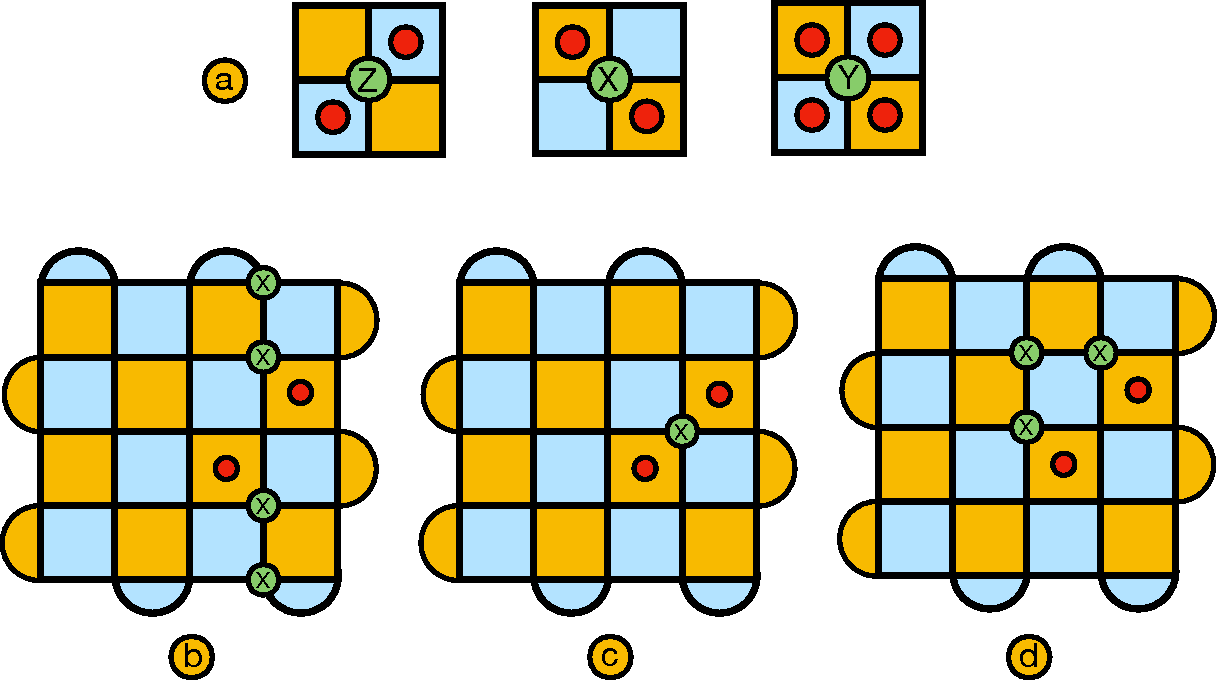
\includegraphics[width=1\linewidth]{figures/surface_code_examples.pdf}
	\caption{
		(a) Single qubit Pauli flips violate surrounding stabilizers.
		(b-d) Strings of Pauli flips only violate stabilizers at the endpoint of the string.
		Multiple error configurations can give rise to the same syndrome.
		They can differ by stabilizers, as for example in (c) and (d), or by logical operators, see (b) and (c).}
		\label{f:surface_code_examples}
	\end{figure}
	In addition to the inherent difficulty resulting from syndrome ambiguity, in experimental settings the process of extracting the syndrome is also subject to noise, and hence the syndrome itself may be faulty \cite{tomita2014low,stephens2014fault}.
	In practice, each stabilizer is associated with a physical ancilla qubit.
	The syndrome value for that particular stabilizer is obtained by first executing a small quantum circuit which entangles the ancilla with each of the physical data qubits on which the corresponding stabilizer is supported.
	The syndrome value is then extracted via a measurement of the ancilla qubit.
	In order to fully account for errors during the process of syndrome extraction one should therefore model this entire circuit, in which errors can occur on both the data qubits and ancilla qubits at each time step.
	Moreover, errors on the ancilla qubits can propagate onto the data qubits via the required entangling gates.

	\begin{figure*}
	\centering
	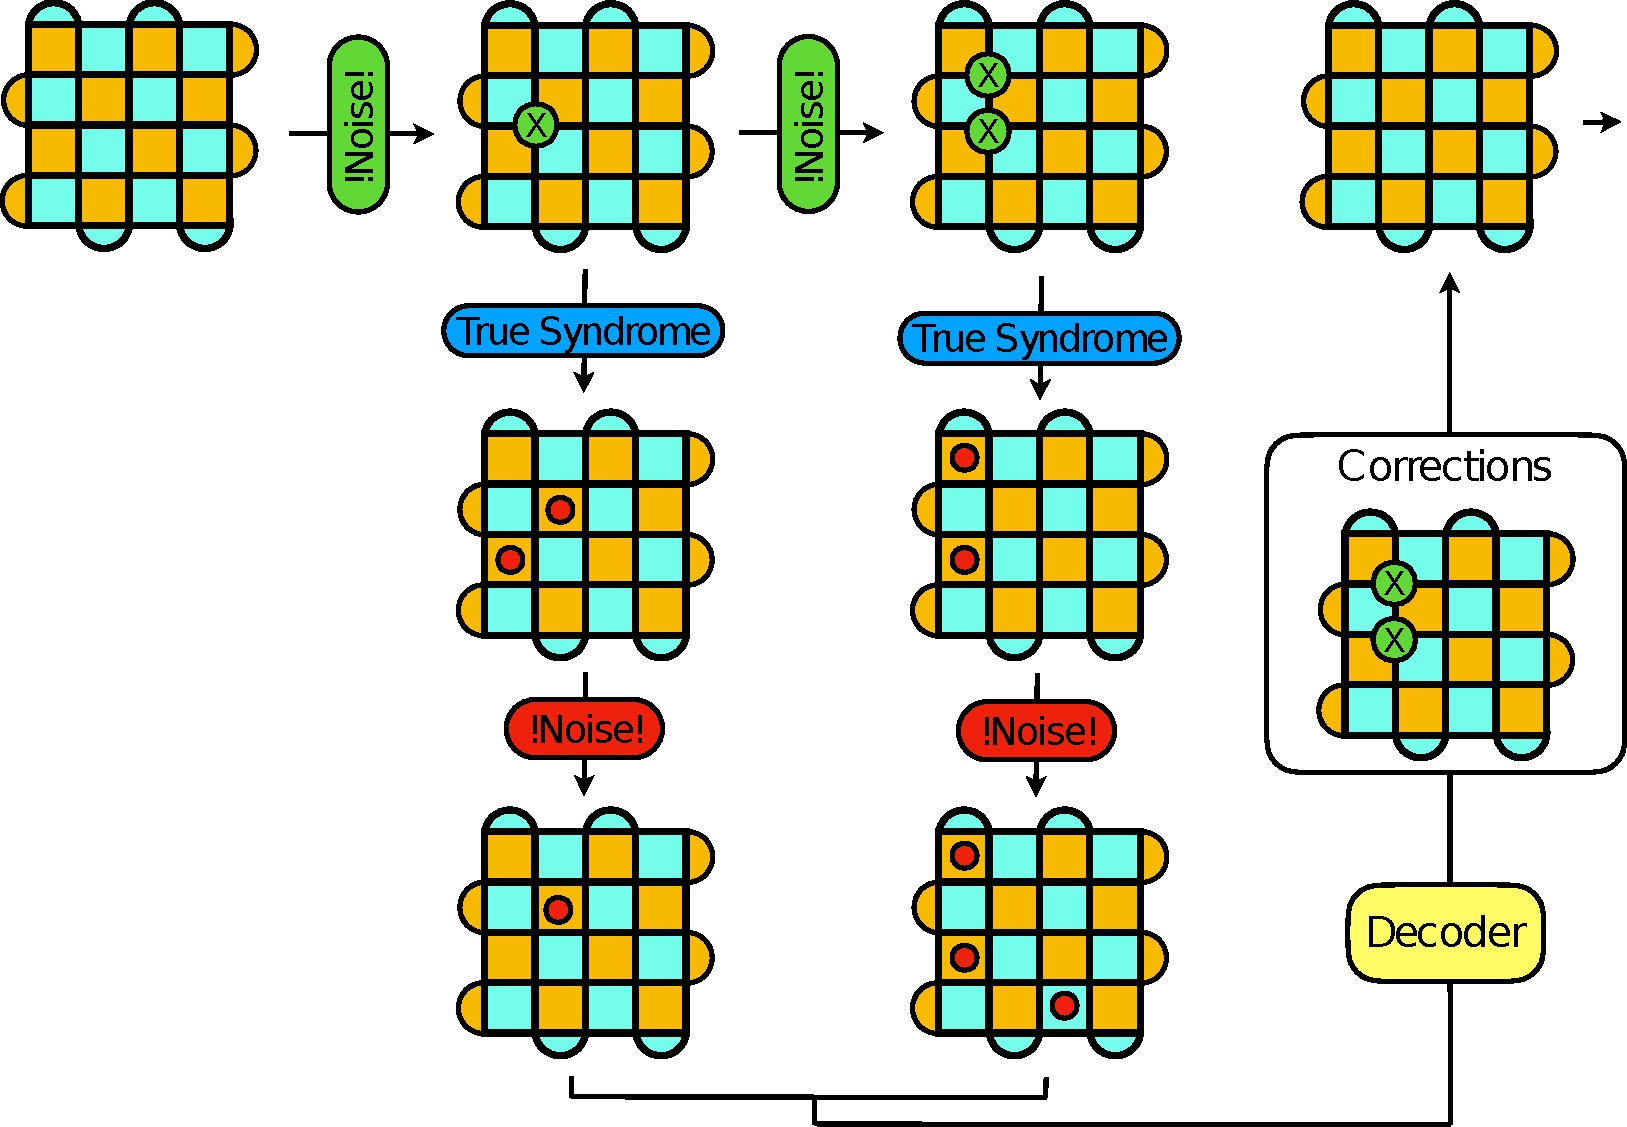
\includegraphics[width=0.6\textwidth]{figures/decoding_problem.pdf}
	\caption{
		A typical decoding cycle is illustrated for the simplified faulty measurements scenario in which one imagines each time step consisting of an initial physical error process generating errors on the data qubits, followed by a second measurement error process which corrupts the true syndrome.
		The decoding algorithm then has access to a sequence of potentially faulty syndromes.}\label{f:decoding_problem}
	\end{figure*}

	The essential aspect of the additional difficulty from faulty syndrome measurements can be phenomenologically modelled by imagining each time step as consisting of two distinct error processes \cite{stephens2014fault}, as illustrated in Fig.~\ref{f:decoding_problem}.
	In the first error process, an error occurs on each data qubit with some probability.
	One then imagines extracting the perfect syndrome before a second error process occurs, in which with a given probability an error occurs on each stabilizer measurement outcome.
	In this scenario, single syndrome measurements are hence no longer reliable.
	Decoding in the fault tolerant setting therefore typically requires providing a set of sequential syndrome measurements.

	Finally, in the context of surface code based fault tolerant quantum computing, all logical gates are implemented either via protocols which also involve an inherent decoding procedure or do not spread errors.
	To be specific, it is sufficient for universal quantum computing to be able to implement both Clifford and $T$ gates~\cite{Nebe01,Bravyi05}.
	In contemporary proposals for surface code based quantum computing~\cite{Litinski18b,Fowler18} protocols are known for implementing Clifford gates either by tracking, via code deformation~\cite{Brown17} or via lattice surgery~\cite{Horsman12,Litinski18}.
	Code deformation and lattice surgery requires several decoding cycles.
	Non-Clifford gates, such as the $T$ gate, can be performed fault tolerantly via gate teleportation using magic states.
	High quality magic states can be obtained via magic state distillation, which requires only Clifford gates and faulty magic states~\cite{Bravyi05}.
	As such the goal of decoding idling logical qubits within a quantum computation should be to suppress errors to the extent that any of the above procedures can succeed with high probability.
	Therefore, we can relax the requirement that the decoding process should return the post-error state to the initial state in the code space.
	In Section~\ref{s:decoding_as_rl} we discuss a proxy criterion for decoding success within this framework.

\section{Reinforcement Learning and q-Functions}\label{s:reinforcement_learning}

	In this section we shift focus and introduce some of the fundamental concepts of reinforcement learning and $q$-functions, which will be essential to our rephrasing of the decoding problem in Section \ref{s:decoding_as_rl}.
	Again, we will constrain ourselves to the basics and refer to Ref. \cite{RLSutton18} for a complete treatment.
	A generic reinforcement learning problem considers an agent interacting with an environment, as is illustrated in Fig. \ref{f:agent_environment}.
	The agent can act on and observe (parts) of the environment, and is tasked with achieving a problem-specific goal by performing a sequence of actions. 
	We typically consider discrete problems, in  which at each step time step $t$ the environment can be described by a state $S_t \in \mathcal{S}$, where $S$ is referred to as the state space.
	Given a state of the environment, the agent can then choose to perform an action $A_t \in \mathcal{A}$, where $\mathcal{A}$ is referred to as the action space.
	As a result of the agents chosen action, the environment then updates accordingly, entering a new state $S_{t+1}$ and providing feedback to the agent on its choice of action in the form of a scalar reward $R_{t+1}$.
	We will restrict ourselves here to episodic environments, for which there exist a set of terminal states $\mathcal{S}_{\mathrm{terminal}} \subset \mathcal{S}$.
	In such episodic settings, in addition to a scalar reward, the agent also receives a boolean signal indicating whether $S_{t+1} \in \mathcal{S}_{\mathrm{terminal}} $ - i.e. whether or not it is ``game over''.

	In general, the agent's choice of action, the resulting state of the environment and the returned reward can all be stochastic. In the case of finite state and action spaces, the environment can then be formalized via a finite Markov decision process (FMDP);

	\begin{equation}
		p(s',r|s,a) \equiv \mathrm{pr}(S_t = s',R_t = r|S_{t-1} = s, A_{t-1} = a).
	\end{equation}
	To formalize the decision making process of the agent, we define an agent's \textit{policy} $\pi$, in essence the agent's strategy, as a mapping from states to probabilities of specific actions - i.e. $\pi(a|s)$ is the probability that agent chooses $A_t = a$, given that the environment is in state $S_t = s$.
	For FMDP's we then define the \textit{value} of a state $s$ under policy $\pi$ as,

	\begin{equation}
		v_{\pi}(s) = \mathbb{E}_{\pi}[G_t|S_t = s]  = \mathbb{E}_{\pi} \Big[\sum_{k = 0}^{\infty}\gamma^k R_{t+k+1}\Big| S_t = s \Big] 
	\end{equation}
	$\forall S_t \in \mathcal{S}$. 
	The term $G_t$ is the discounted return (discounted cumulative reward), with discount factor $0 \leq \gamma \leq 1$, and is the quantity that the agent is tasked with optimizing.
	In episodic settings the infinite sum terminates whenever state $S_{t+k+1}$ is a terminal state - i.e. $S_{t+k+1} \in \mathcal{S}_{\mathrm{terminal}}$.
	We call $v$ the \textit{state-value function}, providing the expected discounted cumulative reward the agent would obtain when following policy $\pi$ from state $s$.
	It is an important conceptual point to note that by using the metric of the discounted cumulative reward the value of any given state depends not only on the immediate reward obtained by following a specific policy from that state, but includes future expected rewards.
	Hence strategies which involve some element of successful future planning may lead to higher state values.
	As such, we see that the value of a state with respect to a given policy reflects accurately the ability of an agent to achieve its long-term goals when following that policy from that state. 

	Similarly to the \textit{state-value function}, we can define the \textit{action-value function}  (referred to as the $q$-function) for policy $\pi$ via:

	\begin{align}
		q_{\pi}(s,a) &= \mathbb{E}_{\pi}[G_t|S_t = s, A_t = a]  \\
		& = \mathbb{E}_{\pi} \Big[\sum_{k = 0}^{\infty}\gamma^k R_{t+k+1}\Big| S_t = s, A_t = a \Big]
	\end{align}
	Clearly, the $q$-function with respect to a given policy is conceptually similar to the state-value function, differing only in that it provides the value for state-action pairs.
	Importantly, value functions allow us to place an order over policies, i.e. $\pi > \pi' \iff v_{\pi}(s) > v_{\pi'}(s)\quad \forall s \in \mathcal{S} $.
	This in turn allows us to define an optimal policy $\pi^*$, for which:

	\begin{figure}
		\centering
		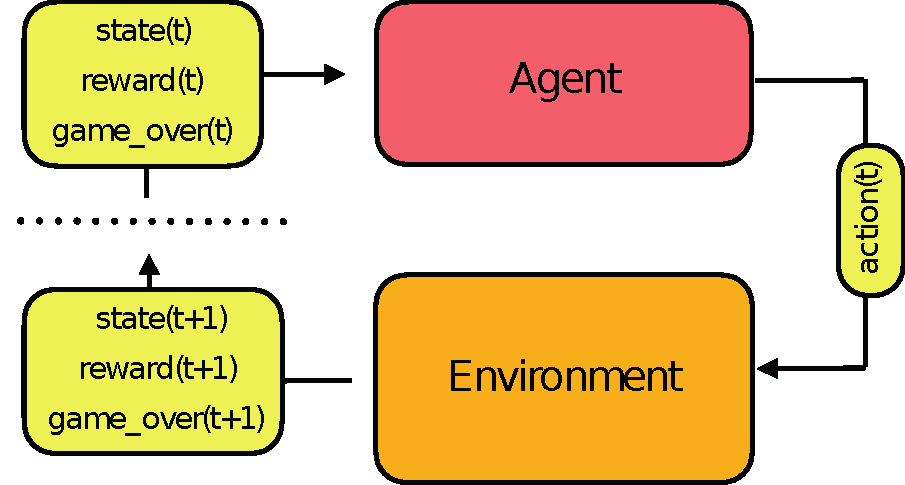
\includegraphics[width=0.4\textwidth]{figures/agent_environment.pdf}
		\caption{
			An illustration of the signals passed between an agent and the environment through the duration of a sequential turn based episode.
		}
		\label{f:agent_environment}
	\end{figure}

	\begin{equation}\label{e:fixed_point}
		q_*(s,a) = \mathbb{E}\big[R_{t+1} + \gamma\max_{a'}q_{*}(S_{t+1},a')\big|S_t = s, A_t = a \big].
	\end{equation}
	Note that given the optimal $q$-function it is easy to obtain the optimal strategy; In a given state $s$ simply choose the action $a = \mathrm{argmax}_{a'}[q_*(s,a')]$.

	Given this framework, there are many different approaches and methodologies that can be used to learn optimal policies.
	We will focus here on $q$-learning, the goal of which is to find or approximate $q_*(s,a)$.
	This is generically done via iterative $q$-learning, in which the agent starts with an arbitrary $q$-function and then iteratively refines it on the basis of experience gained from interaction with the environment.
	In particular, in order to generate such experience, the agent uses a policy derived from its $q$-function (possibly in addition to other explorative policies) to choose actions.
	This $q$-function is then periodically updated using Eq. \eqref{e:fixed_point}, for which $q_*(s,a)$ is a stationary solution \cite{RLSutton18}.

	The above describes concisely the elements of $q$-learning, however it does not address the general impracticality of storing this $q$-function.
	In most real world applications, the number of valid state-action pairs can be impractically large (e.g. consider the number of possible chess configurations).
	It is precisely to address this problem, and in effect to render $q$-learning applicable in practice, that \textit{deepQ} learning was introduced \cite{RLMnih15,RLvan2016deep,RLschaul2015prioritized}.
	In particular, in deepQ learning we parametrize $q$ by a neural network, and use Eq. \eqref{e:fixed_point} to construct the cost function from which the network weights can be updated via a stochastic gradient descent method.
	The learning of the $q$-function is hence done by training a neural network in an online supervised manner, the training instances for which are generated by having the agent explore the environment.
	Specifically, we let the agent interact with the environment via an $\epsilon$-greedy exploration policy, in the process generating experience-tuples of the following form:

	\begin{equation}
		[S_t,A_t,R_{t+1},S_{t+1}]
	\end{equation}
	The set of these tuples then provides an experience memory, from which we can periodically sample a training-batch.
	Given such a batch of training instances, the $q$-network is then updated via the cost function:

	\begin{align} 
		C &= y_{\mathrm{pred}} - y_{\mathrm{true}}\\
		&= q(S_t,A_t) - \big[R_{t+1} + \gamma\max_{a'}q(S_{t+1},a') \big]
	\end{align}
	which, by comparison with Eq.~\eqref{e:fixed_point}, will be minimized only for the optimal policy.
	Unfortunately, despite the simplicity of this idea, in practice a variety of tricks - such as separate active and target $q$-networks, double-$q$ learning and dueling networks - are required to achieve stable $q$-learning.
	We refer to the relevant references \cite{RLMnih15,RLvan2016deep,RLschaul2015prioritized,RLwang2015dueling}, or to the associated code repository \cite{DeepQDecoding}, for details.

\section{Decoding as a Reinforcement Learning Problem}\label{s:decoding_as_rl}

	We now turn to describing the main topic of this work. 
	Namely, we formulate the problem of decoding within the context of \emph{fault-tolerant} quantum computation as a reinforcement learning problem.
	The advantage of this formulation is that it allows for all the methods and techniques of reinforcement learning to be brought to bear on this problem, thereby providing a new toolbox for obtaining diverse \emph{decoding agents}, a novel class of decoding algorithms.
	To present this formulation, we will describe a single episode, as illustrated in Fig. \ref{f:single_episode}.

	At a high level, the environment is constructed from the surface code and the action space of the agent consists of all single qubit Pauli $X$ or $Z$ flips, along with an identity action. 
	A single episode starts with the extraction of a sequence of faulty syndromes and ends whenever errors have accumulated to the extent that a subsequent logical operation is likely to fail, in a sense that will be made precise below.
	Specifically, as shown in Fig. \ref{f:single_episode} (a),  the initial step ($t=0$) of any episode, in which the initial state $S_1$, reward $R_1$ and terminal state indicator $T_1$ are generated, proceeds according to the following steps;

	\begin{figure*}
		\centering
		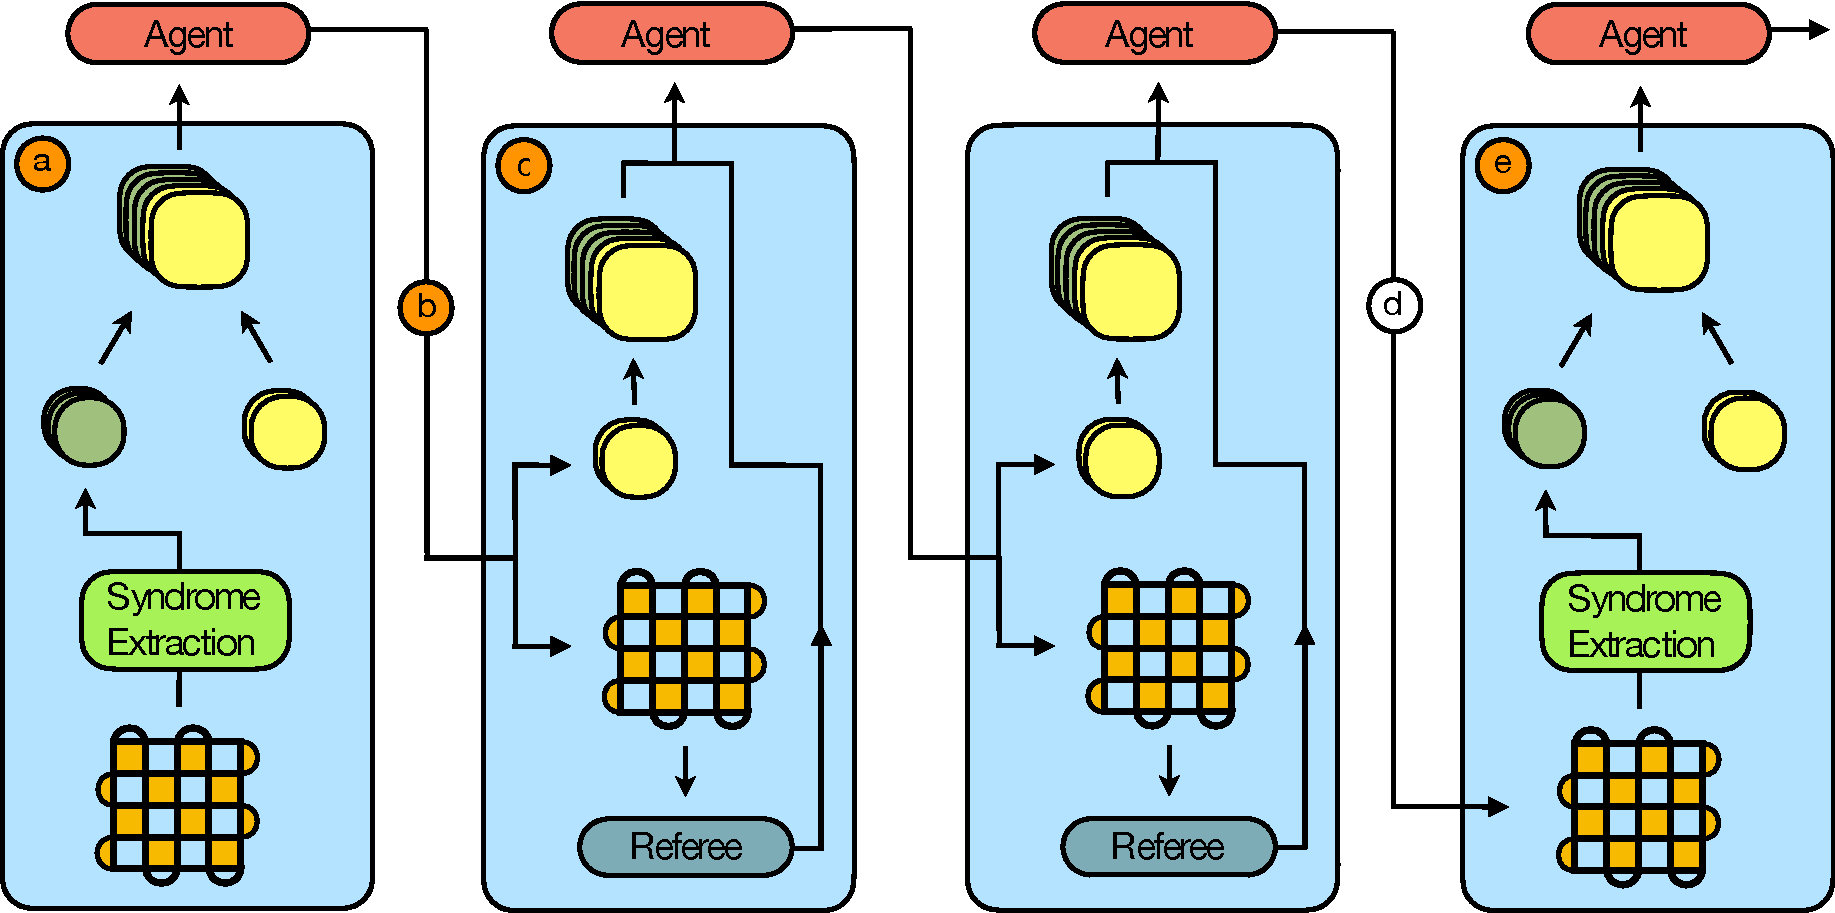
\includegraphics[width=0.65\textwidth]{figures/decoding_as_rl.pdf}
		\caption{
			An illustration of the various steps occurring within a single episode.
			(a) In an initial step, a faulty syndrome volume is extracted from a state initially in the code space.
			This faulty syndrome volume is combined with an initially empty action history and passed to the agent as the initial state.
			Given an input state, the agent must decide on an action, which it passes to the environment.
			If the action is neither an identity or a repetition of an action already in the action history (b), then the procedure illustrated in box (c) occurs, if a trivial or already performed action is chosen (d), then the procedure illustrated in box (e) occurs.
			(c) The chosen action is applied to the underlying quantum state.
			From this state the reward for the applied action is determined, while simultaneously a referee decoder decides whether or not the episode is now over - i.e.
			whether the underlying quantum state is now in a terminal state.
			Additionally, the applied action is appended to the action history, which is concatenated with the non-updated syndrome volume and provided to the agent, in conjunction with the reward and terminal state indicator.
			(e) Once again, the underlying quantum state is first updated, and from this updated state both a reward and terminal state indicator are determined (not shown).
			However, the trivial or repeated action of the agent triggers a new round of faulty syndrome measurements.
			After this new round of syndrome extraction, the new syndrome volume is combined with a reset action history and provided to the agent, from which it can once again choose another move.
		}
		\label{f:single_episode}
	\end{figure*}

	\begin{enumerate}
		\item First, the state of the system (consisting of physical data qubits), which we will refer to as the \textit{hidden state} of the environment, is initialized to some logical state $|\psi_0\rangle \in \mathcal{H_\mathrm{sc}}$.
		The agent's task will be to preserve this state.
		Since this state is in the code space by construction, it can be simply represented as an empty list representing a code lattice on which no Pauli flips have been applied to any physical data qubits.
		\item Then an initial sequence of faulty syndromes is generated.
		We utilize the two-stage error process involving separated physical and measurement errors, as described in Fig.~\ref{s:the_decoding_problem}.
		We wish to emphasise however that in principle a circuit model for syndrome extraction could also be simulated.
		The errors on physical data qubits which were generated during the syndrome extraction protocol are then added to the hidden state of the environment, since we will need them later to evaluate the agent's choice of actions. 
		The agent has no knowledge of, or direct access to, this hidden state.
		\item The visible aspect of the environment, which the agent can observe, is then constructed from the sequence of faulty syndromes, illustrated by the green slices in Fig.~\ref{f:single_episode}.
		We will refer to this sequence of faulty syndromes as the \emph{syndrome volume}, denoted $S_{E,1}$.
		In addition to the syndrome volume, the total state received by the agent at any time step also contains a list of the actions taken by the agent since the last new syndrome volume was received, which we illustrate in Fig.~\ref{f:single_episode} with the yellow slices and refer to as the action history $h$.
		Since for this first step a new syndrome volume was just extracted, the action history of the agent is reset - i.e. $h_1$ is an empty list -  and this reset action history is combined with the syndrome volume and provided to the agent as the total output state of the environment - i.e. $S_1 = (S_{E,1},h_1)$.
		\item The agent has not yet taken any actions, so the reward for this first step is $R_1 =0$. 
		Additionally, in order to allow the episode to continue the terminal state indicator to false - i.e. $T_1=0$.
	\end{enumerate}

	After this initial step, we now need to perform step $t=1$.
	In general, as illustrated in Fig.~\ref{f:agent_environment}, given the state $S_t$, the agent needs to choose an action $A_t$ to apply to the environment, after which the environment needs to respond with the tuple $(S_{t+1}, R_{t+1}, T_{t+1})$, where $S_{t+1}=(S_{E,{t+1}},h_{t+1})$.
	Depending on the action chosen by the agent, the environment can respond in one of two ways, illustrated in Fig.~\ref{f:single_episode} (c) and (e) respectively.

	\subsection{Non-identity and non-repeated actions}

		If, as shown in Fig. \ref{f:single_episode} (c), the agent chooses any non-identity action that is not already an element of the action history list $h_t$, then this step of the episode continues via the following process;

		\begin{enumerate}
			\item Firstly, given the chosen non-trivial action $A_t$, the first step is to apply this action to the code lattice - i.e. the agents chosen action is added to the hidden state of the environment, which is now a combination of all actions and errors on physical data qubits.
			\item The environment now needs to determine the reward $R_{t+1}$ the agent should receive for its action, and whether resulting hidden state is a terminal state.
			As was discussed in Section~\ref{f:decoding_problem}, within the context of surface code based fault tolerant quantum computation the goal of the decoding process for idling logical qubits should be to suppress errors to the extent that future logical operations (which either involve decoding cycles of their own or do not spread errors) can succeed with high probability.
			As such, if after application of the agent's chosen action the current state of the system $|\psi\rangle$ is equal to the original state $|\psi_0\rangle$ - or equivalently, if all errors have been corrected without implementing a logical operation - we give the agent a reward of $+1$, i.e. $R_{t+1} = +1$.
			In all other cases we set $R_{t+1} = 0$, giving the agent no reward.
			\item In addition to the above, we introduce a separate \emph{referee} decoder to act as a proxy for future logical operations.
			This referee decoder should be a ``single-shot" decoder which, given a single perfect syndrome, suggests corrections which always move the current state back into the code space.
			However, this referee decoder may fail by inadvertently performing a logical operation.
			After the hidden state of the environment is updated to include the agents chosen action, this referee decoder is then given a perfect syndrome extracted from the state $|\psi\rangle$ corresponding to the current hidden state.
			If the referee decoder is able to correctly decode this perfect syndrome then the hidden state is not a terminal state, and $T_{t+1} = 0$.
			If on the other hand the referee decoder is not able to correctly decode this perfect syndrome, then we set $T_{t+1}=1$, which indicates the end of the episode.
			\item Finally, the new total state of the environment,  $S_{t+1} = (S_{E,t+1},h_{t+1})$, is constructed as follows;
			Firstly, the action history $h_{t+1}$ is obtained by appending $A_t$ to $h_t$.
			Then, as no new syndrome volume was generated in this step, we set $S_{E,{t+1}} = S_{E,t}$.
		\end{enumerate}
		
	\subsection{Identity or repeated actions}

		If on the other hand the agent chooses either the identity action or an action it has already chosen, then the environment responds via the following procedure, as illustrated in Fig.~\ref{f:single_episode} (e).

		\begin{enumerate}
			\item If the action $A_t$ is a non-identity action which is already in the action history - i.e. $A_t \in h_t$, then the first step is to apply the action to the code lattice by appending the action to the hidden state. In this case, the reward $R_{t+1}$ and terminal state indicator $T_{t+1}$ are then determined by the procedure already described above, as in steps in which a non-identity action was taken.
			\item If the chosen action was the identity however, then this hidden state update is not necessary, and given that the previous hidden state could not have been a terminal state we set $T_{t+1} = 0$, before setting $R_{t+1} = R_t$, as the hidden state has not changed.
			\item Now, we interpret the performing of an identity (either explicitly via the identity action or implicitly by repeating a correction twice) by the agent as a request for a new syndrome, and hence a new syndrome volume is generated.
			Similarly to the initial step of the episode, the hidden state is then updated to include the errors on physical data qubits introduced via this syndrome extraction.
			Additionally, the action history $h_{t+1}$ is once again reset to an empty list, while the visible state $S_{E,t+1}$ is updated to reflect the newly extracted syndrome volume.
			Finally, the total output state $S_{t+1} = (S_{E,t+1},h_{t+1})$ is returned to the agent.
		\end{enumerate}
	

	At this stage we have all the ingredients required to obtain decoding agents through the application of a variety of reinforcement learning algorithms.
	In Section~\ref{s:dq_agent} we will present a detailed construction for a deepQ agent, that allows us to apply deepQ learning and obtain decoding agents whose
	performance is shown in Section~\ref{s:results}.
	Before proceeding however it is worthwhile to emphasize a few points;

	\begin{figure*}
	\centering
	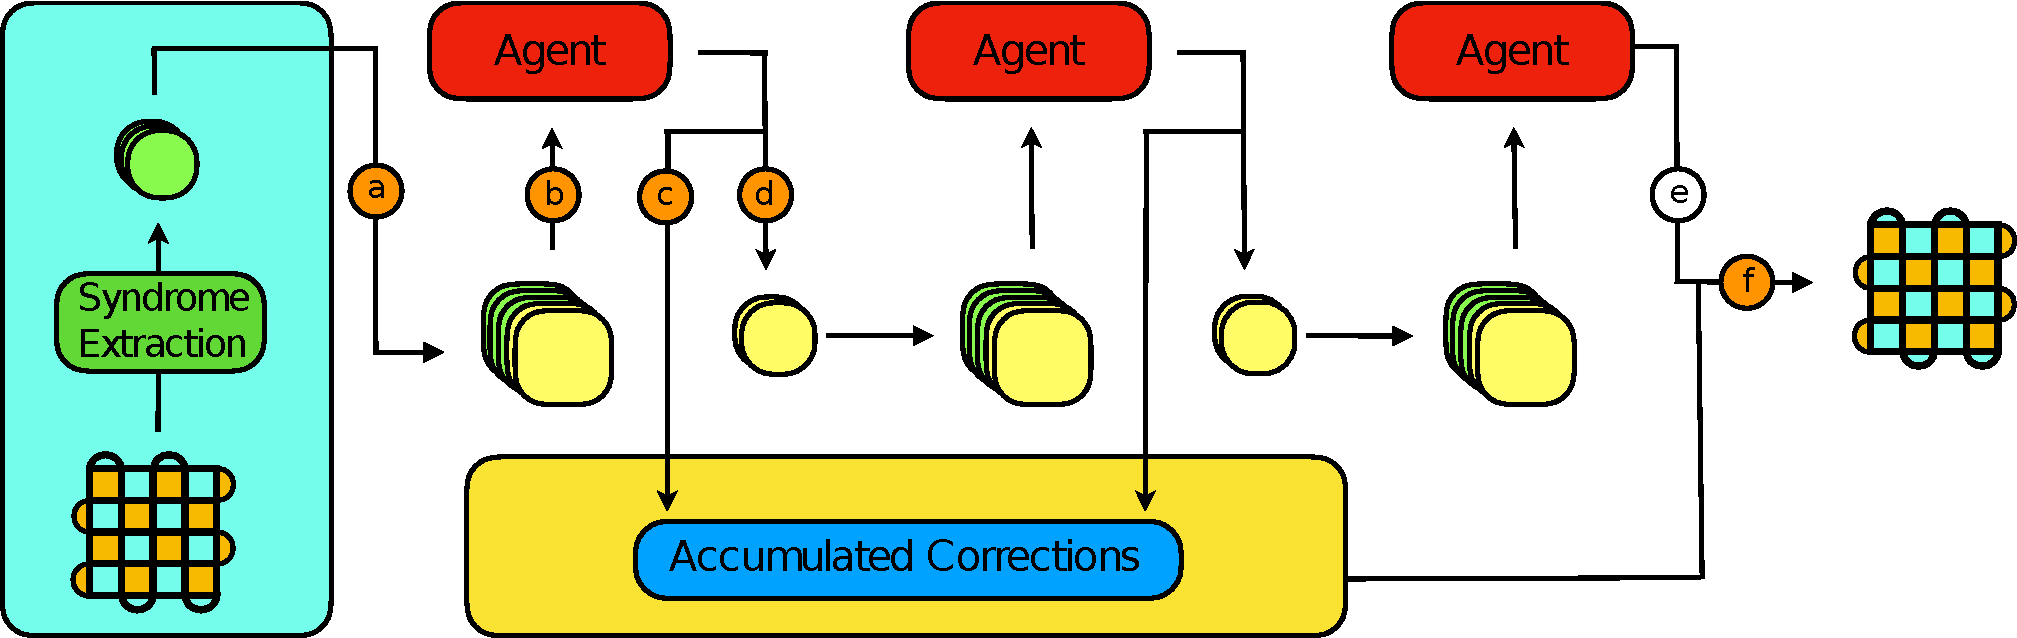
\includegraphics[width=0.7\textwidth]{figures/agent_decoding.pdf}
	\caption{The procedure for decoding with a trained agent.
			(a) Given a faulty syndrome volume generated by some experiment, this volume is concatenated with an empty action history to produce a suitable input state for the decoding agent.
			(b) The decoding agent takes in the combined faulty syndrome volume and action history and chooses an action.
			This action is simultaneously (c) added to a list of accumulated corrections and (d) used to update only the action history component of the input state to the agent.
			This updated input state is then given to the agent and procedures (b-d) continue until the agent (e) repeats an action or chooses the identity.
			(f) At this stage the corrections could be applied to the lattice state, although in practice they would be tracked through the entire computation.
		}
		\label{agent_decoding}
	\end{figure*}

	First, it is important to note that the above agent-interaction framework is both code and error model agnostic, provided one has access to a referee decoder, capable of single-shot decoding on perfect syndromes.
	From this perspective, one might view the framework presented here as a tool for leveraging single-shot, perfect-syndrome decoding algorithms, into decoding algorithms for the fully fault-tolerant setting.
	Additionally, it should be clear from the rules via which rewards are assigned, that the agent will only accumulate reward provided it can learn to consistently correct any errors that might occur on physical data qubits, without implementing logical operations.
	However, the agent is \textit{not} constrained to return the state back into the code space between successive syndrome measurements.
	In particular, because typical reinforcement learning algorithms take into account not only immediate rewards, but rather discounted cumulative rewards, the agent may learn strategies involving actions whose benefit may not be immediate.
	For example, if a rare event occurs and multiple measurement errors occur within the extraction of a syndrome volume, creating a highly ambiguous and difficult to decode input state, the agent may choose to only partially decode before requesting a new syndrome volume, in which hopefully less measurement errors will occur and the underlying error configuration may be less ambiguous.
	As such, the decoding agents obtained via this framework may have access to truly novel decoding strategies, that are not currently available to alternative decoding algorithms.

	It is also useful to note that in practice it is possible to speed-up learning by utilizing various improvements.
	First of all, when choosing exploratory actions, we can restrict the action space to a reduced set of potentially valid corrections.
	In particular, the agent need only consider actions on vertices either involved in a violated stabilizer or adjacent to vertices which have already been acted on.
	This restriction effectively increases the probability of the agent discovering useful actions, and therefore the effectiveness of any exploration phase.
	Second, when generating new syndrome volumes, we discard those cases in which the syndrome is trivial.
	In these cases, the agent does not need to act and hence no useful experience tuple would be generated.
	This allows any experience memory required by the learning algorithm to consist of only useful memories.

	Finally, although we have now thoroughly addressed a framework to which reinforcement learning algorithms could be applied to \textit{train} an agent, we have not yet explicitly discussed the implementation of our $q$-function based agent and how it may be used to decode within an experimental setting.
	As illustrated in Fig.~\ref{agent_decoding}, the latter problem is straightforwardly addressed.
	Given a faulty syndrome volume from an experiment, we initialize an empty action history list and combine this with the faulty syndrome volume as an initial input to the decoding agent.
	The trained agent can then be asked directly for an initial correction, which is added to a list of accumulated corrections.
	Simultaneously \textit{only} the action history element of the previous input state is updated.
	This updated input state, containing the original syndrome volume and the subsequently performed corrections, is then given again to the agent as input.
	This process is iterated until the agent either repeats a correction or chooses the identity, which should be taken as a signal to perform another round of syndrome measurements.

\section{A deepQ Decoding Agent}\label{s:dq_agent}

	\begin{figure*}
		\centering
		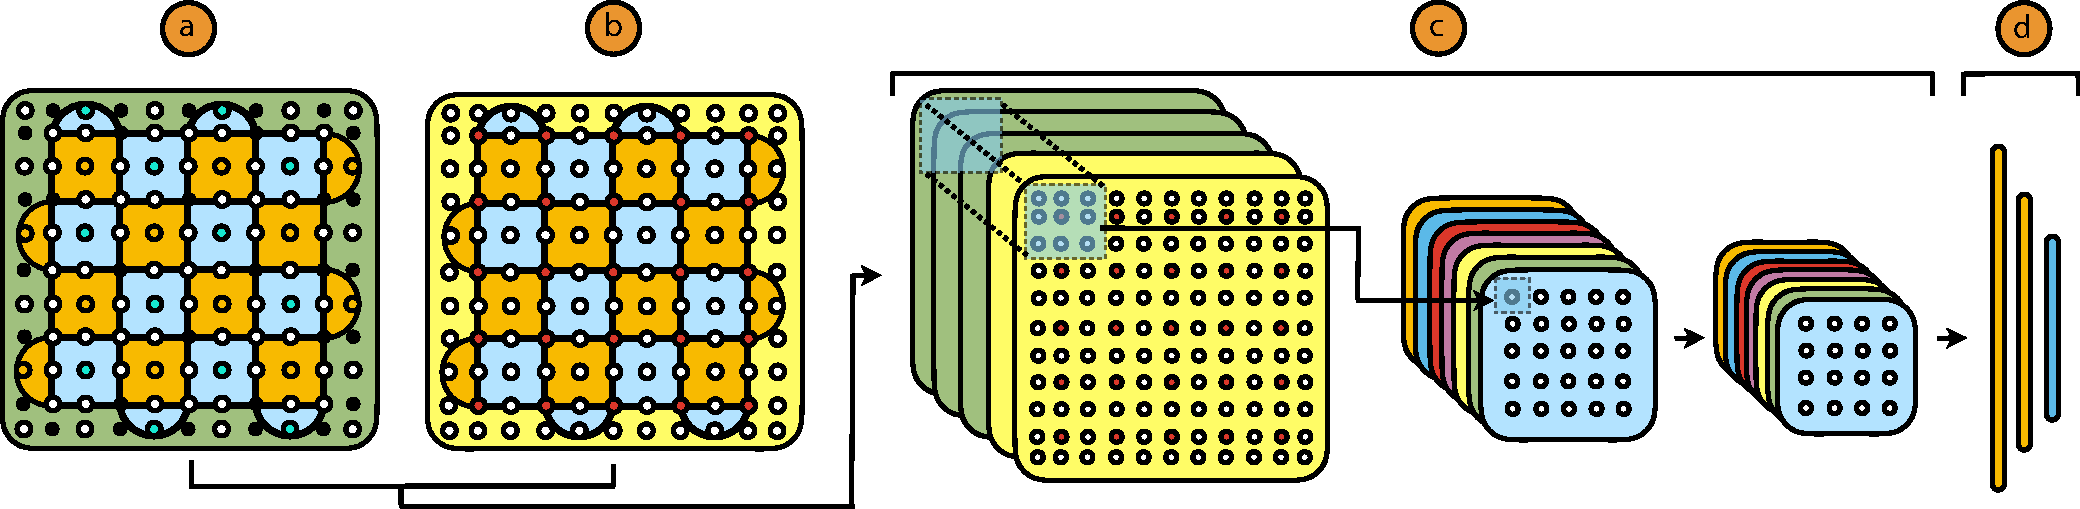
\includegraphics[width=0.9\textwidth]{figures/agent.pdf}
		\caption{
			Details of a deepQ decoding agent for a $d\times d$ code lattice.
			(a) A single faulty syndrome is embedded into a $(2d +1)\times(2d+1)$ binary matrix, where by default all entries are initially set to $0$.
			Entries indicate by orange (blue) circles are then used to indicate violated $Z$ ($X$) stabilizers on the corresponding plaquette.
			Entries indicated by black circles are set to $+1$ as a way of differentiating different types of stabilizers.
			(b) Using the same embedding, the action history for $Z$ ($X$) flips can be encoded by indicating a previous flip on a specific vertex qubit via the entry corresponding to that vertex.
			(c) By stacking the syndrome and action history slices, the total state $S_t$ can be constructed in a form suitable for input to a convolutional neural network.
			(d) To complete the deepQ network, we stack a feed forward neural network on top of the convolutional layers.
			In particular, the final layer of this network has $|\mathcal{A}|$ activations, each of which encodes $q(S_t,a)$ for an action $a$.
		}
		\label{f:agent}
	\end{figure*}

	As discussed in the previous section, many different reinforcement learning algorithms could now be applied within the framework presented here. 
	However, in order to provide a concrete example and proof-of-principle, we will specialize to deepQ learning, which has been previously utilized to obtain agents capable of human-level control in domains such as Atari.
	As mentioned briefly in Section~\ref{s:reinforcement_learning}, a variety of now standard tricks are required to get deepQ learning to work in practice, and we will not present these details here, referring the reader to the relevant references \cite{RLMnih15,RLvan2016deep,RLschaul2015prioritized,RLwang2015dueling} or associated code repository \cite{DeepQDecoding}.
	However, there are various details concerning the construction of the deepQ agent which may be useful for applying alternative deep reinforcement learning algorithms within this framework, and as such we will present these details in this section.

	In particular, in Section~\ref{s:decoding_as_rl} we described how at the beginning of any time step $t$ the agent is supplied with the state $S_{t}=(S_{E,{t}},h_{t})$, where $S_{E,{t}}$ needs to be constructed from a faulty syndrome volume, and $h_{t}$ is a representation of the agents action history.
	In deepQ learning, and in many other deep reinforcement learning algorithms, this state $S_t$ needs to be provided as the input to a deep neural network.
	For example, in the case of deepQ learning, the state $S_t$ is the input to the deepQ network parametrizing the $q$-function from which the agent is partially deriving its policy.
	As such, utilizing an appropriate encoding of $S_t$, which allows for the use of appropriate neural networks, is important.

	In Fig.~\ref{f:agent} we have illustrated the encoding of $S_t$ which was used to facilitate the use of deep convolutional neural networks to parametrize the $q$-function.
	In particular, as shown in Fig.~\ref{f:agent} (a) and (b), we can embed a $d\times d$ code lattice into a $(2d + 1)\times(2d+1)$ binary matrix, where each entry corresponds to either a plaquette, a vertex, or an edge of the lattice.
	As shown in Fig.~\ref{f:agent} (a), we can then use a single such binary matrix to encode each of the faulty syndromes, by using the entries corresponding to plaquettes to indicate violated stabilizers, and the remaining entries to differentiate both blue and orange, and bulk and boundary plaquettes.
	Similarly, as illustrated in  Fig.~\ref{f:agent} (b) we can use two such binary matrices to encode the action history, by using one matrix to indicate the physical data qubits on which $X$ flips have already been applied, and the other binary matrix to indicate the data qubits on which $Z$ flips have already been applied.
	As can be seen in Fig.~\ref{f:agent} (c), the total state $S_t$ can then be obtained by stacking the action history slices on top of the faulty syndrome slices, effectively creating a multi-channel image suitable as input for a convolutional neural network.
	In particular, the strength of this encoding is that any convolutional filter, such as the one indicated in Fig.~\ref{f:agent} (c), then isolates all relevant information, both violated stabilizers and applied actions, from some local patch of the lattice.
	Finally, the deepQ network we utilize is completed by stacking a feed forward neural network on top of multiple convolutional layers.
	In particular, the final layer of this network has $|\mathcal{A}|$ activations, each of which encodes $q(S_t,a)$ for an action $a$.

\section{Results}\label{s:results}

	As a demonstration, we utilized deepQ learning within the framework presented in Section~\ref{s:decoding_as_rl}, to obtain deepQ decoding agents for both bit-flip and depolarizing noise, with faulty syndromes, for a $d=5$ surface code lattice.
	All the code utilized to obtain these agents is supplied in the corresponding \textit{DeepQ-Decoding} code repository \cite{DeepQDecoding}, and as such we will provide only an overview of the details here.
	In particular, for a single fixed set of hyper-parameters, we used the original deepQ algorithm \cite{RLMnih15}with annealed $\epsilon$-greedy exploration, implemented via the keras-RL library \cite{plappert2016kerasrl} and incorporating doubleQ updates \cite{RLvan2016deep} and dueling networks \cite{RLwang2015dueling}.
	In addition we used a custom training procedure, described in Appendix~\ref{A:training}, for sequentially iterating through increasing error rates, while simultaneously performing a hyper-parameter grid search at each error-rate iteration.
	For both error models we utilized a convolutional deepQ network, as illustrated in Fig.~\ref{f:agent}, consisting of three convolutional layers, followed by a single feed-forward layer before the final output layer.
	Specifically, if we describe a single convolutional layer with a three-tuple $[n,w,s]$, where $n$ is the number of filters, $w$ is the filter width and $s$ is the stride, and a single feed forward layer via a two-tuple $[n,d]$, where $n$ is the number of neurons and $d$ is the output drop-out rate, then from input to output our deepQ networks had the structure,


	\begin{equation}
		[[64,3,2],~[32,2,1],~[32,2,1],~[512,0.2],~[|\mathcal{A}|, 0]],
	\end{equation}
	where $|\mathcal{A}|$ is the size of the action space.
	All other additional hyper-parameters used to obtain each decoding agent, along with histories of each training procedure, are provided in Appendix~\ref{A:parameters}.

	\begin{figure*}
		\centering
		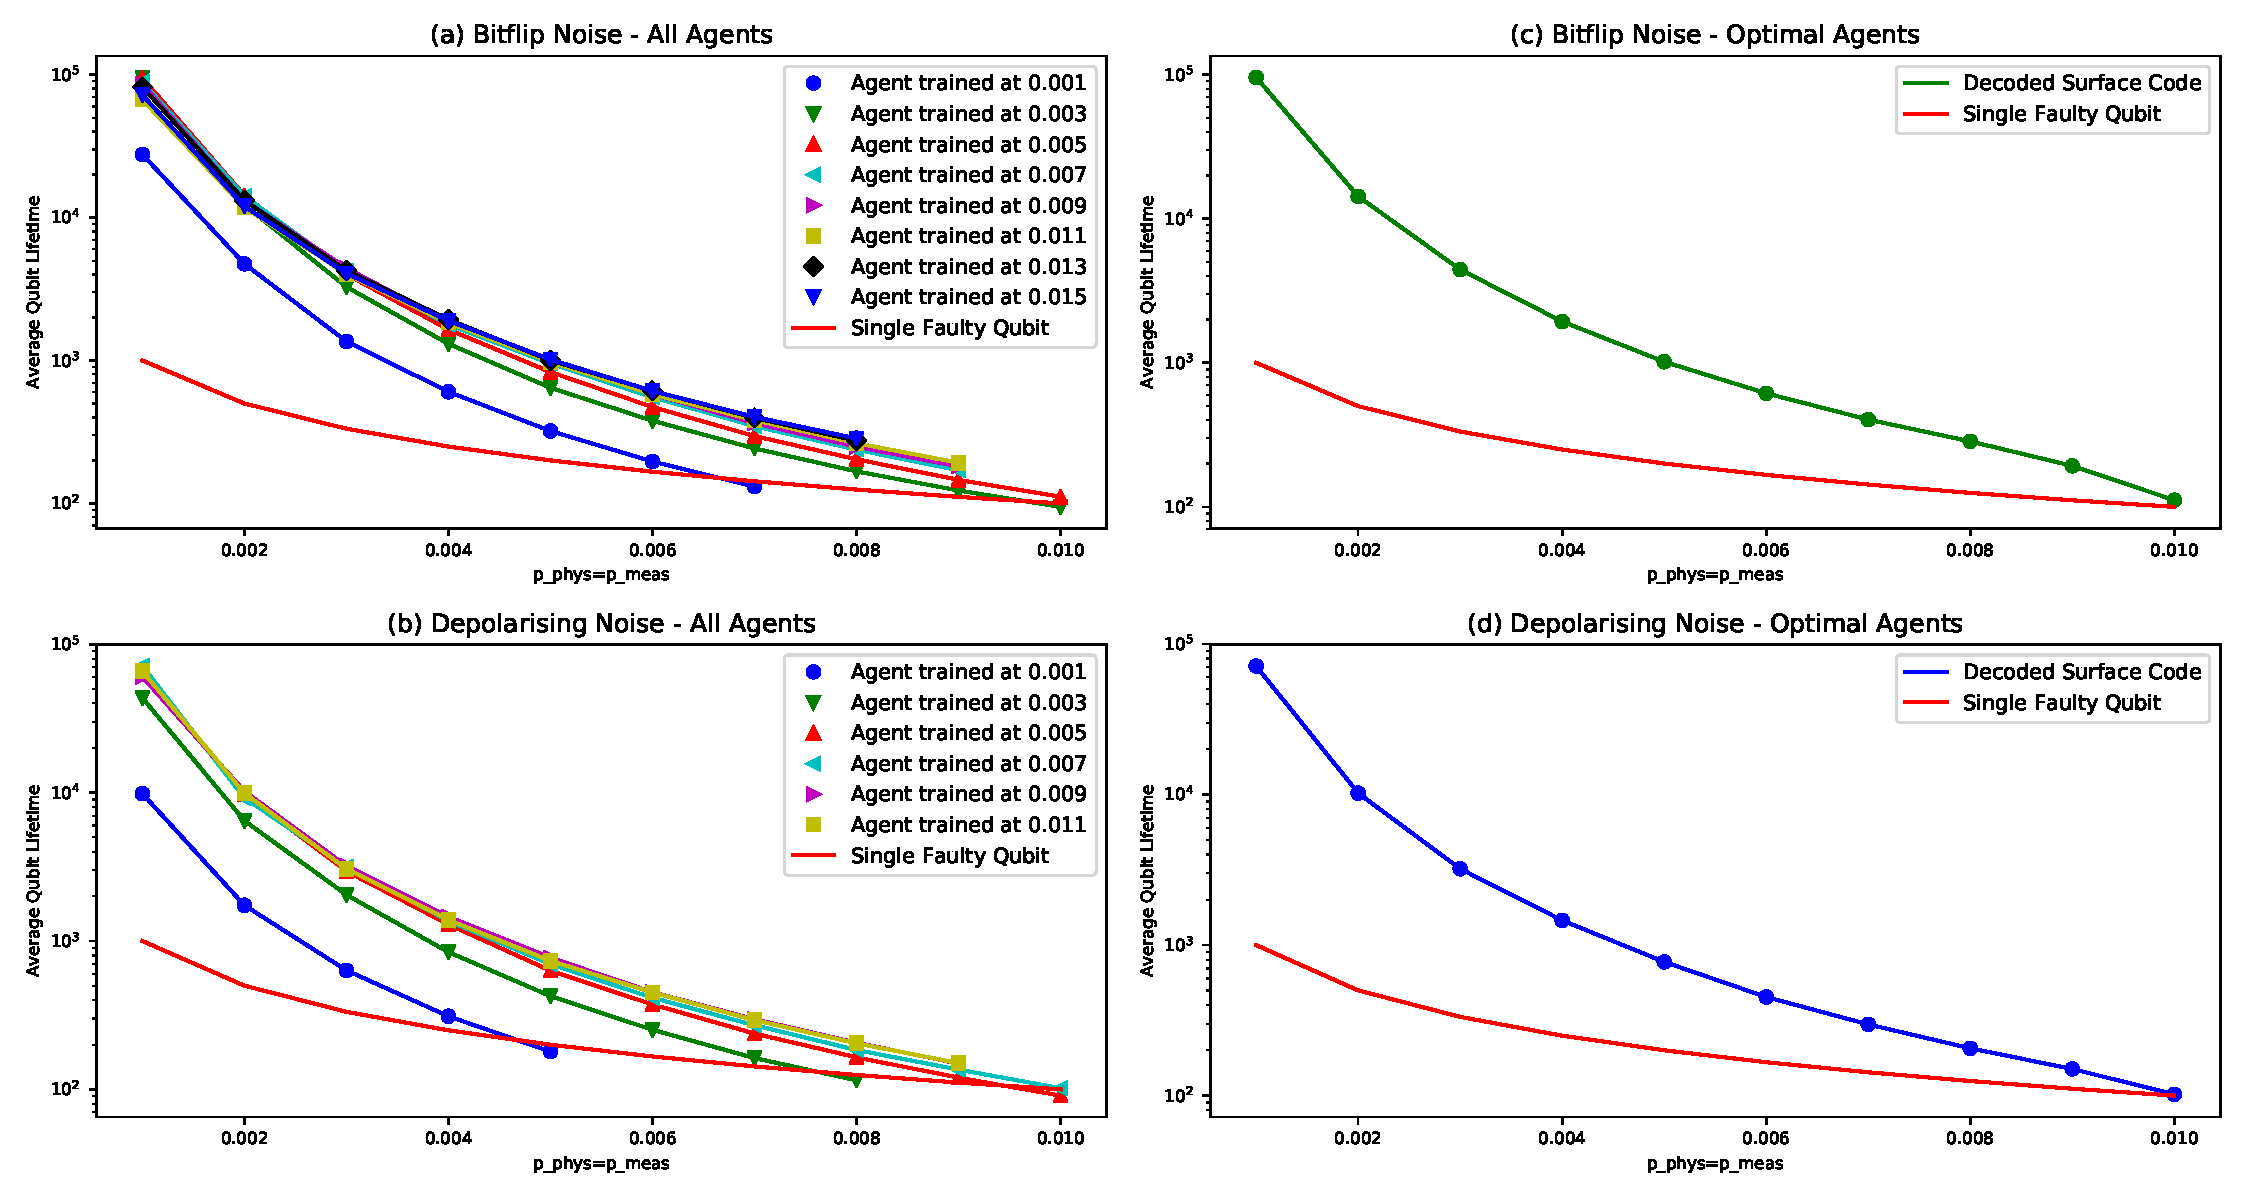
\includegraphics[width=\linewidth]{figures/final_results.pdf}
		\caption{(a,b) Performance of all agents obtained during the iterative training procedure. Each agent was evaluated at increasing error rates, until the average lifetime of the logical qubit actively decoded by the agent became less than the average lifetime of a single faulty qubit. (c,d) Results obtained by using the optimal decoding agent for each error rate.}\label{f:results}
	\end{figure*}

	We then considered both bit-flip and depolarizing noise.
	For both error models we considered the measurement of a single syndrome to consist of two separate error channels, as illustrated in Fig.~\ref{f:decoding_problem}.
	For bit-flip noise, in the first error channel - the physical error channel - a Pauli $X$ flip was applied to each physical data qubit with probability $p_{\mathrm{phys}}$.
	For depolarising noise, the physical error channel acted by applying to each physical data qubit, with probability $p_{\mathrm{phys}}$, either a Pauli $X$, $Y$ or $Z$ flip, with equal probability.
	For both noise models, after the physical error channel, the true syndrome was calculated, after which the second measurement error channel was applied, in which the value of each stabilizer measurement was flipped with probability $p_{\mathrm{meas}}$.
	For all simulations we set $p \equiv p_{\mathrm{phys}} = p_{\mathrm{meas}}$.
	Also, note that for bit-flip noise, as only $X$ corrections were necessary, we had $|\mathcal{A}| = d^2 + 1$ - i.e. the agent could perform either the identity or a single qubit $X$ flip on any individual physical data qubit.
	For depolarising noise, we restricted the agent to only $X$ and $Z$ flips (as $Y$ errors can be corrected via both an $X$ flip and a $Z$ flip), such that $|\mathcal{A}| = 2d^2 + 1$.

	To evaluate the performance of our trained decoders we used the procedure described in Fig.~\ref{agent_decoding}, where the agent selected actions via the final $q$-function in a purely greedy manner, with identity or repeated actions triggering new syndrome volumes.
	The referee decoder was used to check after every action of the agent whether or not a terminal state had been reached, and the length of a single episode was reported as the number of individual syndromes seen by the agent (i.e. the number of times the two-fold error channel was applied) before a terminal state was reached.
	For each error rate, the average lifetime of the actively decoded logical qubit was determined by the average episode length, over a number of episodes that guaranteed at least $10^6$ syndromes were seen by the decoding agent.
	This average logical qubit lifetime was then compared with the average lifetime of a single faulty qubit.

	The final results are then shown in Fig. \ref{f:results}.
	In particular, Fig. \ref{f:results} (a, b) shows the performance of all decoding agents obtained during the iterative training procedure (as described in Appendix \ref{A:training}), while Fig. \ref{f:results} (c, d) shows the results obtained by the using the optimal decoding agent for each error rate.
	For bit-flip (depolarising) noise we find that for approximately $p < 1.3\times 10^{-2}$  $(p < 1.1\times 10^{-2})$ there is a decoding agent for which the average lifetime of the actively decoded logical qubit is longer than the average lifetime of a single faulty qubit.
	These results are however by no means rigorous thresholds, and are meant as a demonstration and proof-of-principle. 
	In this regard there are various points worth emphasising.

	Firstly, both the neural network architecture and reinforcement learning algorithm used here are comparatively simple with respect to the current state-of-the-art \cite{RLmnih2016asynchronous,RLSilver17b,RLsilver2017mastering,RLSilver2016}, and were chosen to allow for the execution of the required training procedure with the available computational resources.
	As such, it is expected that utilization of either more sophisticated neural network architectures or learning algorithms, coupled with the computational resources required for implementing the required training procedures, could allow one to obtain significantly better results.
	Furthermore, as discussed in ref. \cite{chamberland2018deep}, using dedicated hardware it is expected that the forward pass time of various applicable neural network architectures (including the architecture used here) can be brought below the time-scales necessary for near-term experiments. 
	This, coupled with the ability to straightforwardly apply the techniques here to circuit-level noise, renders decoding agents such as the ones shown here promising candidates for near-term fault-tolerant experiments.

\section{Conclusion}\label{s:conclusions}

	We have shown that the problem of decoding within the setting of fault-tolerant quantum computation can be naturally reformulated as a reinforcement learning problem.
	In particular, we have provided an agent-environment framework which allows for the application of diverse reinforcement learning algorithms, and provided a proof-of-principle demonstration by training deepQ decoding agents for the $d=5$ surface code, for both bit-flip and depolarizing noise, with faulty syndrome measurements.
	However, this framework is both code and error model agnostic, and as such could be used to obtain decoding agents, a novel class of flexible decoding algorithms, for a wide variety of experimentally relevant settings.
	Additionally, the recent use of more sophisticated reinforcement learning techniques and neural network architectures to demonstrate super-human performance in complex domains such as Chess and Go \cite{RLSilver17b,RLsilver2017mastering,RLSilver2016}, strongly indicate that the initial results presented here, via deepQ learning with small neural networks, could be successfully improved and extended, given the required computational resources for training.
	This, coupled with the development of dedicated special purpose hardware for the fast implementation of neural networks, suggest that decoding agents could indeed provide a practical solution for decoding in near-term fully fault-tolerant quantum computation.

	As a result, there are various natural avenues for extension of this work. 
	First and foremost it would be of interest to explore the performance of alternative decoding agents, obtained via different reinforcement learning algorithms, for a wider class of codes and error models.
	Simultaneously, in the perfect-measurements setting, recent effort has focused on developing techniques to allow for the scaling of neural network decoders to larger code distances \cite{Ni18}
	As such, it would be natural to explore the extent to which these developments could be utilized within the framework presented here, to facilitate obtaining decoding agents for significantly larger code distances.
	Finally, due to the inherent design of the procedure via which these decoding agents are obtained, in which discounted future performance is valued over immediate rewards, these agents have the potential to learn decoding strategies not available to alternative decoding algorithms.
	Hence, it may be possible that analysis of the strategies learned by decoding agents could aid the development of other new decoding algorithms.
	


% Acknowledgments
	\begin{acknowledgments}
		The authors gratefully acknowledge helpful and insightful discussions with Daniel Litinski, Nicolas Delfosse, Aleksander Kubica, Thomas Jochym-O'Connor, Paul Baireuther, and Hendrik Poulsen Nautrup.
		Additionally, the authors would like to thank J\"{o}rg Behrmann for incredible technical support, without which this work would not have been possible.
		RS\ acknowledges the financial support of the Alexander von Humboldt foundation.
		MSK\ is supported by the DFG (CRC183, project B02).
		EvN\ is supported by the Swiss National Science Foundation through grant P2EZP2-172185.
		JE\ is supported by DFG (CRC 183, EI 519/14-1, and EI 519/7-1), the ERC (TAQ), the Templeton Foundation, and the BMBF (Q.com).
	\end{acknowledgments}

\appendix

\section{Distributed Iterative Training with Simultaneous Hyper-Parameter Optimization}\label{A:training}

	In order to obtain optimal decoders for multiple error rates we implemented a custom iterated training procedure, involving a hyper-parameter grid search at each error rate, as illustrated in Fig. \ref{f:iterative_training}. All code for implementing this procedure on an HPC cluster can be found in the associated \emph{DeepQ-Decoding} repository \cite{DeepQDecoding}. In particular, this procedure involves the following steps:

	\begin{enumerate}
		\item Choose an initial error rate $p_1$, and fix the values for any hyper-parameters which should remain constant throughout the entire training procedure.
		\item For all hyper-parameters not yet fixed, specify a list of values to be used for training - i.e. specify a hyper-parameter grid over which one would like to search for an optimal hyper-parameter configuration.
		\item Train multiple decoding agents at the initial error rate, one for each hyper-parameter configuration in the specified grid. Each agent is initialized with an empty experience memory and random initial neural network weights. The training of all agents can be done simultaneously in a distributed manner.
		\item Given the results from all agents trained at $p_1$, sort the results and store the neural network weights and experience memory from the optimal decoding agent.
		\item Increase the error rate to $p_2$. Once again, train multiple decoding agents, one for each hyper-parameter configuration in the specified grid. However, this time all agents are initialized with the experience memory and neural network weights from the optimal agent at $p_1$.
		\item Iterate this procedure until a specified final error rate $p_n$, or until the performance of the optimal agent is worse than that of a single faulty qubit.
	\end{enumerate}

	\begin{figure}
		\centering
		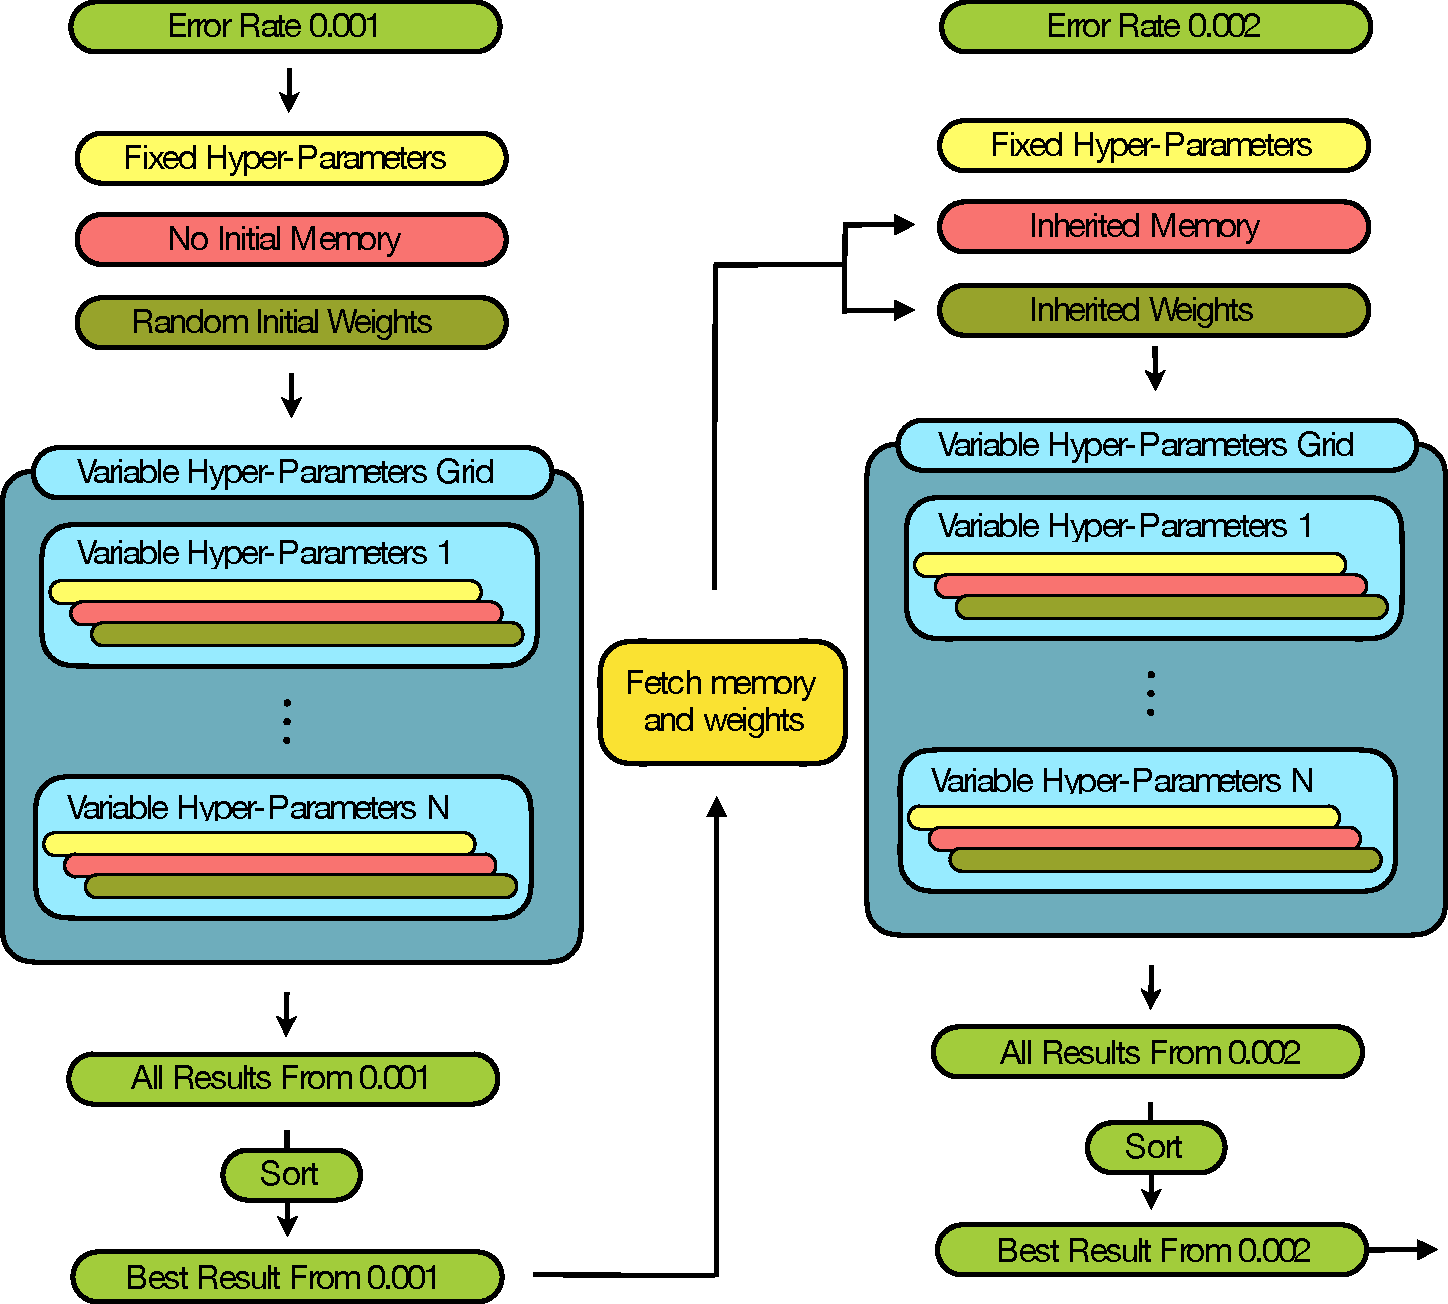
\includegraphics[width=\linewidth]{figures/iterative_training.pdf}
		\caption{Iterative training procedure, via a hyper-parameter grid search at each error rate. After training multiple decoding agents at a given error rate, one for each point in the specified hyper-parameter grid, the results are sorted. The weights and experience memory from the optimal decoding agent are then used as the initial weights and experience memory for a new round of training procedures, again one for each point in the hyper-parameter grid, but at an increased error rate.}\label{f:iterative_training}
	\end{figure}

\section{Agent Hyperparameters and Learning Curves}\label{A:parameters}

	We implemented the distributed iterative training procedure described in Appendix \ref{A:training}, for both bit-flip and depolarising noise (all utilized code can be found in the \emph{DeepQ-Decoding} repository \cite{DeepQDecoding}).
	In particular, the initial error rate was set to $p_1 = p_{\mathrm{phys}} = p_{\mathrm{meas}} = 1\times10^{-3}$, and incremented by $2\times10^{-3}$ in each iteration. 
	The neural network architecture was as described in Section \ref{s:results}.
	All agents were trained via the original deepQ algorithm \cite{RLMnih15}, implemented via the keras-RL library \cite{plappert2016kerasrl}, with annealed $\epsilon$-greedy exploration, doubleQ updates \cite{RLvan2016deep} and dueling networks \cite{RLvan2016deep}.
	Both the fixed hyper-parameters and variable hyper-parameter grids utilized during the training procedure are specified in Table. \ref{t:hyper_parameters}.
	Figs. \ref{f:training_results_dp} and \ref{f:training_results_x} then show the training history of the optimal decoding agent at each error rate, while the associated values for the variable hyper-parameters are given in Table \ref{t:agent_hyper_parameters}.

	\begin{table}
	\begin{center}
	  \begin{tabular}{| c | c | }
	    \hline
	    \multicolumn{2}{|c|}{Fixed Hyper-Parameters} \\
	    \hline
	    Batch size & $32$  \\ 
	    Rolling average length & $1\times10^3$ \\ 
	    Stopping patience (in episodes) & $1\times10^3$  \\
	    Maximum training steps & $1\times10^6$  \\ 
	    Memory buffer size & $5\times 10^4$ \\ 
	    Syndrome volume depth & $5$ \\
	    Discount factor $\gamma$ & 0.99 \\
	    \hline
	    \multicolumn{2}{|c|}{Variable Hyper-Parameters} \\
	    \hline
	    Initial $\epsilon$ & $\{1, 0.5, 0.25\}$ \\ 
	    Final $\epsilon$ & $\{0.04, 0.02, 0.001\}$  \\
	    Number of exploration steps & $\{1,2\}\times10^5$  \\ 
	    Learning rate (LR)& $\{10,5,1,0.5\}\times10^{-5}$  \\ 
	    Target network update frequency & $\{2500, 5000\}$ \\ 
	    \hline
	  \end{tabular}\caption{Training Hyper-Parameters}\label{t:hyper_parameters}
	\end{center}
	\end{table}

	\begin{table}
	\begin{center}
	  \begin{tabular}{| c | c | }
	    \hline
	    \multicolumn{2}{|c|}{Bitflip Noise} \\
	    \hline
	    0.001 & $[2\times10^5,1,0.02,1\times10^{-5},5000]$  \\ 
	    0.003 & $[2\times10^5,1,0.02,1\times10^{-5},5000]$  \\ 
	    0.005 & $[1\times10^5,0.25,0.001,1\times10^{-5},2500]$  \\ 
	    0.007 & $[1\times10^5,1,0.02,1\times10^{-5},5000]$  \\ 
	    0.009 & $[1\times10^5,0.5,0.04,1\times10^{-5},5000]$  \\ 
	    0.011 & $[2\times10^5,0.5,0.04,1\times10^{-5},2500]$  \\ 
	    0.013 & $[1\times10^5,0.5,0.001,1\times10^{-5},5000]$  \\ 
	    0.015 & $[2\times10^5,0.25,0.04,1\times10^{-5},2500]$  \\ 
	    \hline
	    \multicolumn{2}{|c|}{Depolarising Noise} \\
	    \hline
	    0.001 & $[2\times10^5,1,0.001,5\times10^{-5},5000]$  \\ 
	    0.003 & $[1\times10^5,0.25,0.02,1\times10^{-5},5000]$  \\ 
	    0.005 & $[2\times10^5,0.5,0.001,1\times10^{-5},5000]$  \\ 
	    0.007 & $[1\times10^5,1,0.02,1\times10^{-5},5000]$  \\ 
	    0.009 & $[2\times10^5,1,0.02,1\times10^{-5},2500]$  \\ 
	    0.011 & $[2\times10^5,1,0.02,5\times10^{-6},2500]$  \\ 
	    \hline
	  \end{tabular}\caption{Hyper-parameters for optimal agents at each error rate, in the form [\textit{number of exploration steps, initial} $\epsilon$ \textit{, final} $\epsilon$\textit{, learning rate, target network update frequency}]}\label{t:agent_hyper_parameters}
	\end{center}
	\end{table}

	\begin{figure}
		\centering
		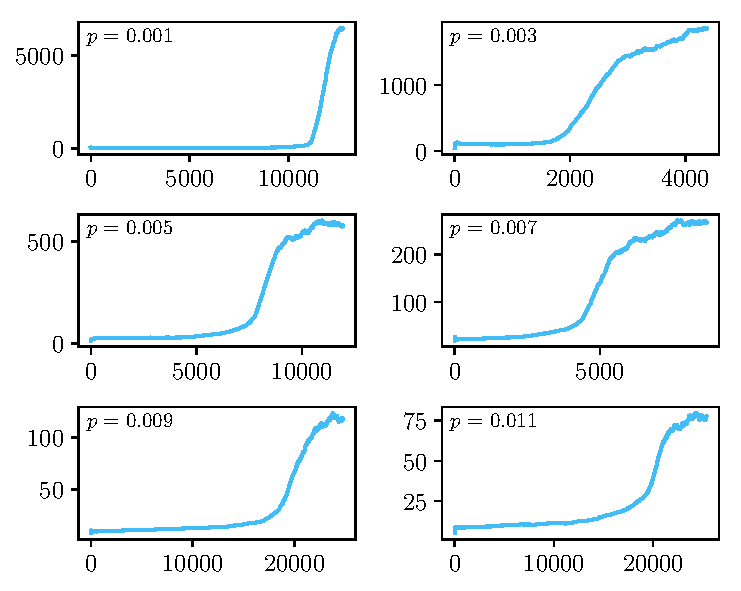
\includegraphics[width=\linewidth]{figures/depolarising_histories.pdf}
		\caption{Training histories for optimal depolarising noise agents. The $x$-axis shows the number of episodes, and the $y$-axis shows the rolling average of the decoded qubit lifetime. Hyper-parameters for each agent are given in Table \ref{t:agent_hyper_parameters}.}\label{f:training_results_dp}
	\end{figure}

	\begin{figure}
		\centering{}
		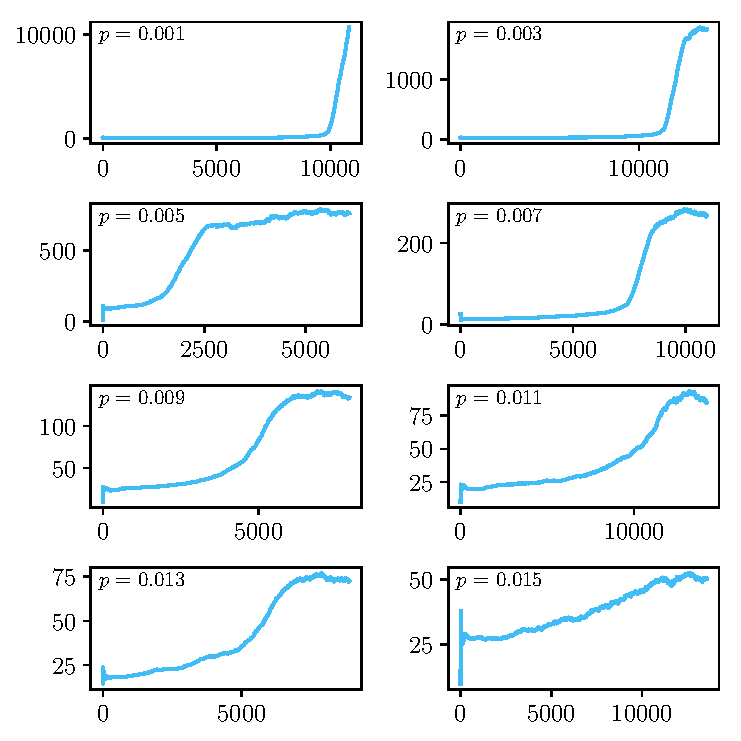
\includegraphics[width=\linewidth]{figures/bitflip_histories.pdf}
		\caption{Training histories for optimal bitflip noise agents. The $x$-axis shows the number of episodes, and the $y$-axis shows the rolling average of the decoded qubit lifetime. Hyper-parameters for each agent are given in Table \ref{t:agent_hyper_parameters}.}\label{f:training_results_x}
	\end{figure}

\clearpage
\bibliographystyle{apsrev4-1mod}
\bibliography{dq}

\end{document}